\documentclass[dvipsnames]{article}
\usepackage{pgfplots}
\usetikzlibrary{decorations.markings}
\pgfplotsset{compat=newest}

% \def\Point{36.9}

\begin{document}

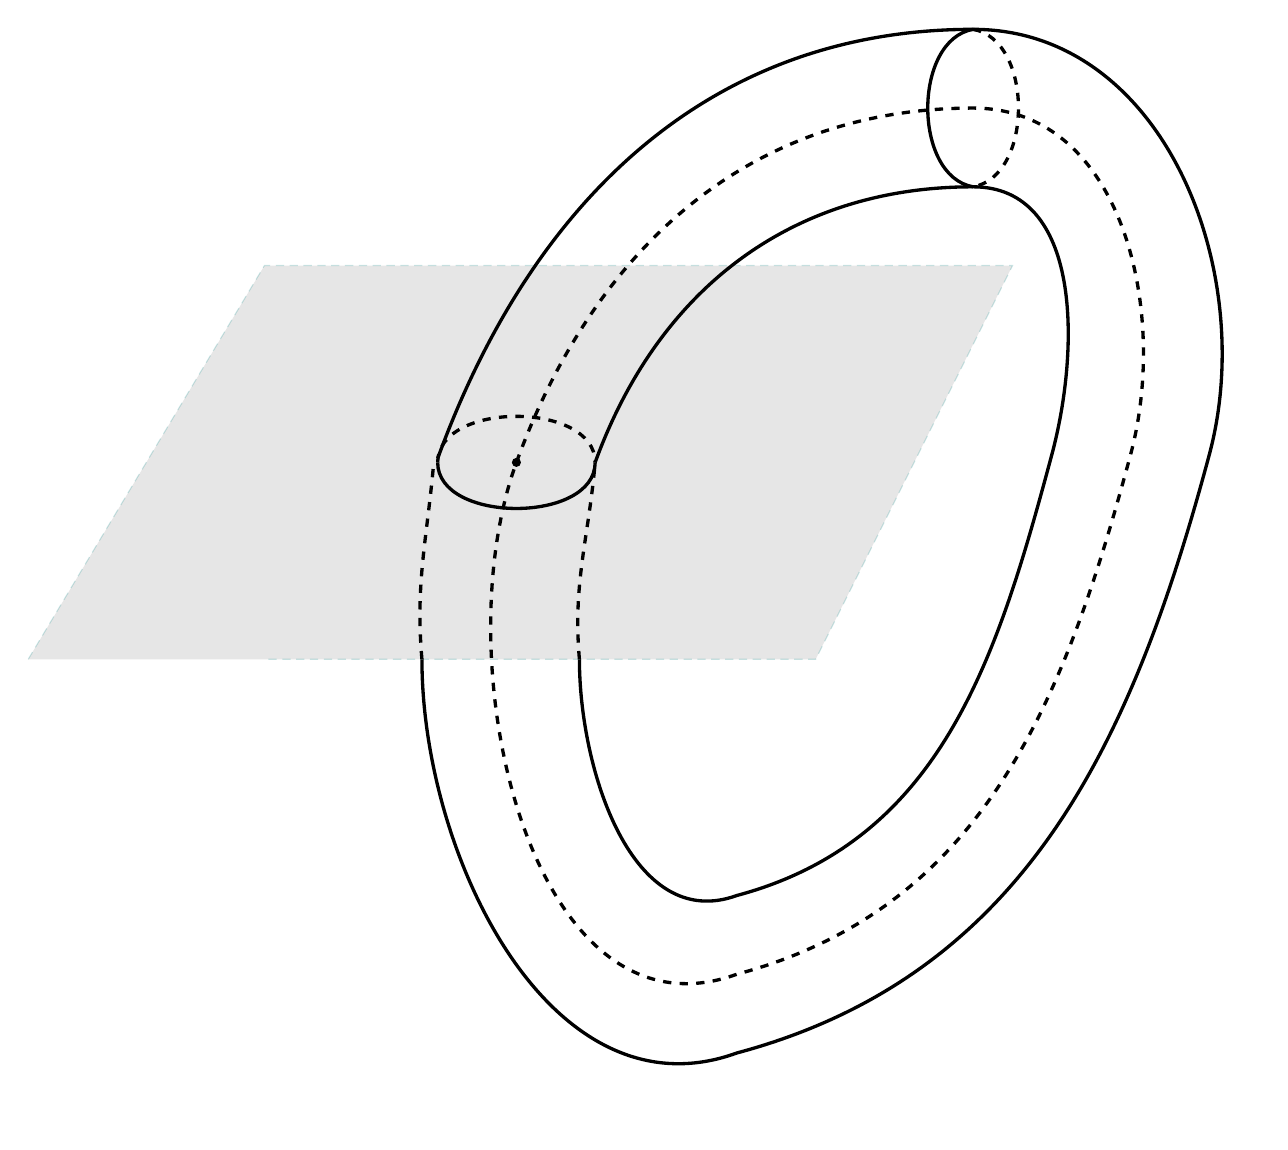
\begin{tikzpicture}
  %плоскость
  \draw[teal,densely dashed][fill = gray, opacity=0.2]  (-1,-1) -- (2,4) -- (11.5,4) -- (9,-1) -- (2,-1);
  %цикл

  \draw [very thick, dashed] (5.2,1.5) to [out=70,in=-180] (11,6) to [out=0,in=75] (13,1.6) to [out=-105,in=15] (8,-5) to [out=-160,in=-110] (5.2,1.5);
  \draw [very thick, dashed] (4.2,1.5) to [out=90,in=90] (6.2,1.5);
  \draw [very thick] (4.2,1.5) to [out=-90,in=-90] (6.2,1.5);
  \draw [very thick] (6.2,1.5) to [out=70,in=-180] (11,5) to [out=0,in=75] (12,1.6) to [out=-105,in=15] (8,-4) to [out=-160,in=-90] (6,-1);
  \draw [very thick] (4.2,1.55) to [out=70,in=-180] (11,7) to [out=0,in=75] (14,1.6) to [out=-105,in=15] (8,-6) to [out=-160,in=-90] (4,-1);
  \draw [very thick, dashed] (4,-1) to [out=95,in=-95](4.15,1.5);
  \draw [very thick, dashed] (6,-1) to [out=95,in=-95](6.2,1.5);
  \draw [very thick] (11,7) to [out=-170,in=170] (11,5);
  \draw [very thick, dashed] (11,7) to [out=-10,in=10] (11,5);
  \draw [fill] (5.2,1.5) circle [radius=0.05];
\end{tikzpicture}
\end{document}